\chapter{Mengenal Kecerdasan Buatan dan Scikit-Learn}
Buku umum teori lengkap yang digunakan memiliki judul\textit{Artificial intelligence: a modern approach}\cite{russell2016artificial}. Untuk pratikum sebelum UTS menggunakan buku \textit{Python Artificial Intelligence Projects for Beginners}\cite{eckroth2018python}. Buku pelengkap penunjang penggunaan python menggunakan buku \textit{Python code for Artificial Intelligence: Foundations of Computational Agents}\cite{poole2017python}.
Dengan praktek menggunakan python 3 dan editor anaconda dan library python scikit-learn.
Tujuan pembelajaran pada pertemuan pertama antara lain:
\begin{enumerate}
\item
Mengerti definisi kecerdasan buatan, sejarah kecerdasan buatan, perkembangan dan penggunaan di perusahaan
\item
Memahami cara instalasi dan pemakaian sci-kit learn
\item
Memahami cara penggunaan variabel explorer di spyder
\end{enumerate}
Tugas dengan cara dikumpulkan dengan pull request ke github dengan menggunakan latex pada repo yang dibuat oleh asisten riset.

\section{Teori}
Praktek teori penunjang yang dikerjakan :
\begin{enumerate}
\item
Buat Resume Definisi, Sejarah dan perkembangan Kecerdasan Buatan, dengan bahasa yang mudah dipahami dan dimengerti. Buatan sendiri bebas plagiat[hari ke 1](10)
\item
Buat Resume mengenai definisi supervised learning, klasifikasi, regresi dan unsupervised learning. Data set, training set dan testing set.[hari ke 1](10)

\textbf{Penjelasan Teori}
          \\Berikut merupakan penjelasasn resume dari Teori :
          \begin{enumerate}
              \item Definisi AI (Kecerdasan Buatan) : Bagaimana sebuah komputer memiliki kemampuan yang sama dengan manusia yang dapat mengambil keputusan sendiri dari berbagai macam kasus yangn di hadapinya. Contoh: komputer dapat berkomunikasi baik dengan kata, suara, gambar dan lain sebagainya.. Oleh karena itu AI (Kecerdasan Buatan) dapat di sebut sebagai robot/digitalisasi yang dikendalikan oleh sistem komputer untuk dapat menyelesaikan suatu tugasnya sesuai instruksi sistem.

              \item Sejarah AI (Kecerdasan Buatan) : Tahun 1940 - 1950 mulai terbentunya komputer modern Para ilmuan mulai diskusi mengenai bidang sybernetics, matematika, algoritma dan teori jaringan pada tahun 1956, pada tahun yang sama McCarthy mendirikan Konferensi Dartmouth di Hanover, New Hampshire yang menemukan beberapa teori kompleks mengenai jaringan saraf dan pemikiran kreatif pada komputer. dengan demikian Kecerdasan Buatan launching.

              \item Perkembangan AI (Kecerdasan Buatan) : 17 tahun berlalu tepatnya pada tahun 1973 Konferensi tersebut mendanai sebuat penelitian di MIT (universitas di Edinburgh,Stanford dan Carnegie Mellon) yang mana komputer pemrograman mulai membuktikan masalah aljabar , teorema geometris yang menggunakan pehamanan sintaks dan tata bahasa inggris.

              \item Scikit-Learn Supervised Learning : Merupakan pengumpulan data yang berlable serta menyediakan algoritma untuk mendukung penilaian di masa yang akan datang. contoh: Mobil self-driving, chatbots, pengenalan wajah, robot, sistem pakar.

              \item Scikit-Learn Unsupervised Learning : Merupakan pengumpulan data yang tidak berlable salah satunya yakni untuk menguji AI sebagai mana mencari tahu cara memilah bebek dan ayam atau juga menambahkan kategori yang beda.

              \item Scikit-Learn Regresi : Metode analisis statik untuk melihat pengaruh terhadap 2 atau lebih variable. contoh: berat atau gajih.

              \item Scikit-Learn Klasifikasi : Proses pengelompokan benda yang sama dan benda yang beda. Contoh: mengidentifikasi orang tersebut apakah pria atau wanita, orang itu udah mandi atau tidak mandi.

              \item Scikit-Learn Dataset : Konsepnya sama dengan yang ada pada databse hanya saja dataset ini berisi koleksi data table dan data relation.

              \item Scikit-Learn Training Set : Berguna untuk algoritma klasifikasi sebagai contoh neural network, bayesian, decision tree bertujuan untuk membentuk sebuah model classifier.

              \item Scikit-Learn Testing Set : Bertujuan untuk mengukur classifier ketika berhasil melakukan klasifikasi bersifat true.
          \end{enumerate}
\end{enumerate}

\section{Instalasi}
Membuka https://scikit-learn.org/stable/tutorial/basic/tutorial.html. Dengan menggunakan bahasa yang mudah dimengerti dan bebas plagiat. Dan wajib skrinsut dari komputer sendiri.

\paragraph{\textbf Youtube :} https://youtu.be/srzfw6J4ZaM

\begin{enumerate}
\item
Instalasi library scikit dari anaconda, mencoba kompilasi dan uji coba ambil contoh kode dan lihat variabel explorer[hari ke 1](10)

\begin{figure}[ht]
    \centerline{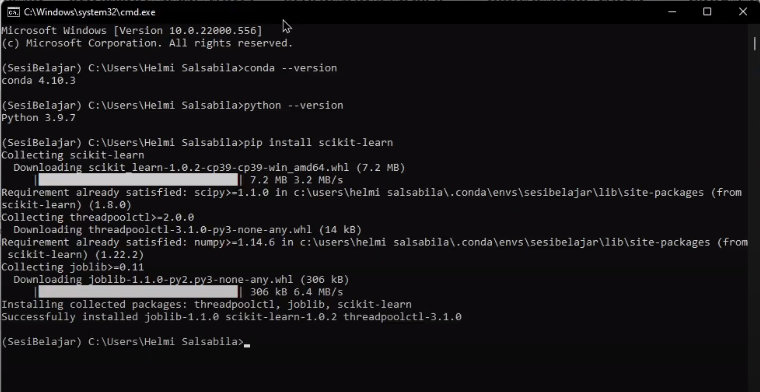
\includegraphics[scale=0.38]{images/Chapter1/Chapter1a.png}
    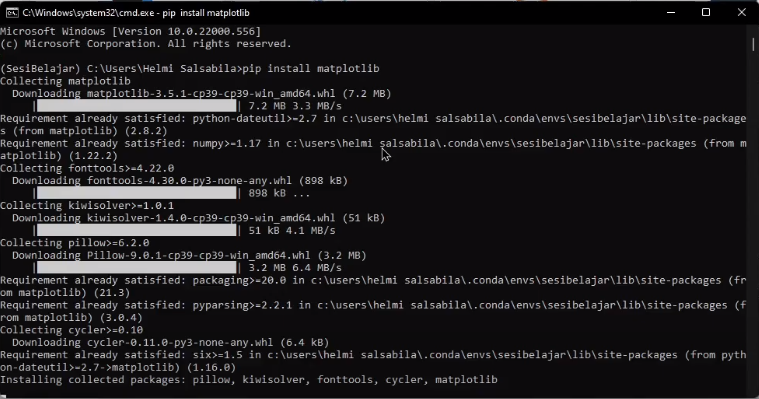
\includegraphics[scale=0.38]{images/Chapter1/Chapter1b.png}}
    \caption{Instalasi Library Scikit-Learn dan Matplotlib}
    \label{Instalasi Library Scikit-Learn dan Matplotlib}
\end{figure}

\item
Mencoba Loading an example dataset, menjelaskan maksud dari tulisan tersebut dan mengartikan per baris[hari ke 1](10)

\begin{figure}[ht]
\centerline{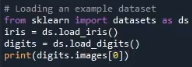
\includegraphics[scale=1]{images/Chapter1/Chapter1c.png}
    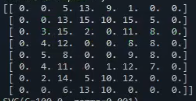
\includegraphics[scale=1]{images/Chapter1/Chapter1ca.png}}
    \caption{Loading an Example Dataset}
    \label{Loading an Example Dataset}
\end{figure}

\item
Mencoba Learning and predicting, menjelaskan maksud dari tulisan tersebut dan mengartikan per baris[hari ke 2](10)

\begin{figure}[ht]
    \centerline{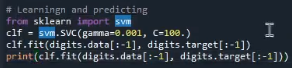
\includegraphics[scale=1]{images/Chapter1/Chapter1d.png}
    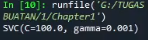
\includegraphics[scale=1]{images/Chapter1/Chapter1da.png}}
    \caption{Learning and Predicting}
    \label{Learning and Predicting}
\end{figure}

\newpage
\item
Mencoba Model persistence, menjelaskan maksud dari tulisan tersebut dan mengartikan per baris[hari ke 2](10)

\begin{figure}[ht]
    \centerline{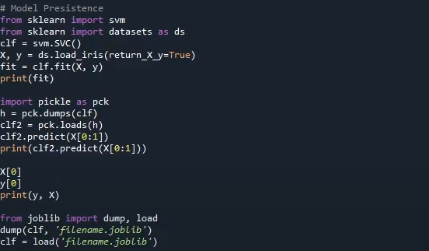
\includegraphics[scale=0.8]{images/Chapter1/Chapter1e.png}
    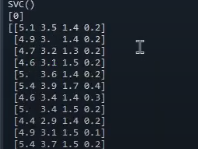
\includegraphics[scale=0.8]{images/Chapter1/Chapter1ea.png}}
    \caption{Model persistence}
    \label{Model persistence}
    \end{figure}

\item 
Mencoba Conventions, menjelaskan maksud dari tulisan tersebut dan mengartikan per baris[hari ke 2](10)

\begin{figure}[ht]
    \centerline{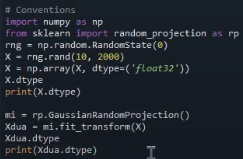
\includegraphics[scale=0.8]{images/Chapter1/Chapter1f.png}
    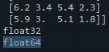
\includegraphics[scale=0.8]{images/Chapter1/Chapter1fa.png}}
    \caption{Conventions}
    \label{Conventions}
    \end{figure}
    
\end{enumerate}

\section{Penanganan Error}
Dari percobaan yang dilakukan di atas, apabila mendapatkan error maka:

\begin{enumerate}
	\item
	skrinsut error[hari ke 2](10)
	
\begin{figure}[ht]
    \centerline{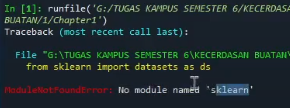
\includegraphics[scale=1]{images/Chapter1/Chapter1error.png}}
    \caption{No module named 'sklearn'}
    \label{ChapterError}
\end{figure}
    
    \newpage
	\item
    Tuliskan kode eror dan jenis errornya [hari ke 2](10)
    \\ Belum mengintal library dari scikit-learn sehingga terjadi error '\textit{No module named sklearn}'
	\item
    Solusi pemecahan masalah error tersebut[hari ke 2](10)
    \\ Instal terlebih dahulu library scikit-learnnya dengan menggunakan terminal yang ada pada anacondanya, kemudian ketikan '\textit{pip install scikit-learn}' tunggu hingga prosesnya selesai dan library sudah bisa di gunakan pada projek anda.
    

\end{enumerate}

